\documentclass[
  bibliography=totoc,     % Literatur im Inhaltsverzeichnis
  captions=tableheading,  % Tabellenüberschriften
  titlepage=firstiscover, % Titelseite ist Deckblatt
]{scrartcl}

% Paket float verbessern
\usepackage{scrhack}

% Warnung, falls nochmal kompiliert werden muss
\usepackage[aux]{rerunfilecheck}

% unverzichtbare Mathe-Befehle
\usepackage{amsmath}
% viele Mathe-Symbole
\usepackage{amssymb}
% Erweiterungen für amsmath
\usepackage{mathtools}

% Fonteinstellungen
\usepackage{fontspec}
% Latin Modern Fonts werden automatisch geladen
% Alternativ zum Beispiel:
%\setromanfont{Libertinus Serif}
%\setsansfont{Libertinus Sans}
%\setmonofont{Libertinus Mono}

% Wenn man andere Schriftarten gesetzt hat,
% sollte man das Seiten-Layout neu berechnen lassen
\recalctypearea{}

% deutsche Spracheinstellungen
\usepackage[main=ngerman]{babel}


\usepackage[
  math-style=ISO,    % ┐
  bold-style=ISO,    % │
  sans-style=italic, % │ ISO-Standard folgen
  nabla=upright,     % │
  partial=upright,   % ┘
  warnings-off={           % ┐
    mathtools-colon,       % │ unnötige Warnungen ausschalten
    mathtools-overbracket, % │
  },                       % ┘
]{unicode-math}

% traditionelle Fonts für Mathematik
\setmathfont{Latin Modern Math}
% Alternativ zum Beispiel:
%\setmathfont{Libertinus Math}

\setmathfont{XITS Math}[range={scr, bfscr}]
\setmathfont{XITS Math}[range={cal, bfcal}, StylisticSet=1]

% Zahlen und Einheiten
\usepackage[
  locale=DE,                   % deutsche Einstellungen
  separate-uncertainty=true,   % immer Fehler mit \pm
  per-mode=symbol-or-fraction, % / in inline math, fraction in display math
]{siunitx}

% chemische Formeln
\usepackage[
  version=4,
  math-greek=default, % ┐ mit unicode-math zusammenarbeiten
  text-greek=default, % ┘
]{mhchem}

% richtige Anführungszeichen
\usepackage[autostyle]{csquotes}

% schöne Brüche im Text
\usepackage{xfrac}

% Standardplatzierung für Floats einstellen
\usepackage{float}
\floatplacement{figure}{htbp}
\floatplacement{table}{htbp}

% Floats innerhalb einer Section halten
\usepackage[
  section, % Floats innerhalb der Section halten
  below,   % unterhalb der Section aber auf der selben Seite ist ok
]{placeins}

% Seite drehen für breite Tabellen: landscape Umgebung
\usepackage{pdflscape}

% Captions schöner machen.
\usepackage[
  labelfont=bf,        % Tabelle x: Abbildung y: ist jetzt fett
  font=small,          % Schrift etwas kleiner als Dokument
  width=0.9\textwidth, % maximale Breite einer Caption schmaler
]{caption}
% subfigure, subtable, subref
\usepackage{subcaption}

% Grafiken können eingebunden werden
\usepackage{graphicx}
% größere Variation von Dateinamen möglich
\usepackage{grffile}

% schöne Tabellen
\usepackage{booktabs}

% Verbesserungen am Schriftbild
\usepackage{microtype}

% Literaturverzeichnis
\usepackage[
  backend=biber,
]{biblatex}
% Quellendatenbank
\addbibresource{lit.bib}
\addbibresource{programme.bib}

% Hyperlinks im Dokument
\usepackage[
  german,
  unicode,        % Unicode in PDF-Attributen erlauben
  pdfusetitle,    % Titel, Autoren und Datum als PDF-Attribute
  pdfcreator={},  % ┐ PDF-Attribute säubern
  pdfproducer={}, % ┘
]{hyperref}
% erweiterte Bookmarks im PDF
\usepackage{bookmark}

% Trennung von Wörtern mit Strichen
\usepackage[shortcuts]{extdash}

\author{%
  AUTOR A\\%
  \href{mailto:authorA@udo.edu}{authorA@udo.edu}%
  \and%
  AUTOR B\\%
  \href{mailto:authorB@udo.edu}{authorB@udo.edu}%
}
\publishers{TU Dortmund – Fakultät Physik}


\title[Toolbox 2025]{Toolbox Workshop 2025}
\subtitle{Python, Unix, Make, Git, \LaTeX{}}
\date{29.~September – 10.~Oktober 2025}
\institute[Pep et al.\ e.V.]{
\includegraphics[height=2cm]{logos/pep.pdf}}
\author[Toolbox Workshop Team]{}

\begin{document}

\maketitle

\begin{frame}{Ziel}
  \setlength\parskip{3ex}
  \huge
  Wir machen euch die Praktikumsprotokolle so einfach, wie möglich.

  Auswerten mit bewährten Methoden.

  Von Anfang an ein zusammenarbeitender Satz an Programmen.

  Auch für die Bachelor-, Masterarbeit wichtig.
\end{frame}

\begin{frame}{Roadmap}
    \begin{center}
      \begin{tikzpicture}[
          >=latex,
          arrow/.style={line width=2pt, ->}
        ]
        %% Data table
        \node at (0, 2.5) {Daten};
        \node (data) at (0, 0) {
          \sffamily
          \sisetup{table-format=1.0, detect-family}
          \begin{tblr}{
              colspec = {S S[table-format=1.3]},
              row{1} = {guard, mode=math},
              row{7} = {guard, mode=math}
            }
            \toprule
            x \mathbin{/} \unit{\milli\metre} & I \mathbin{/} \unit{\micro\ampere} \\
            \midrule
            0 & 0.000 \\
            1 & 0.060 \\
            2 & 0.530 \\
            3 & 1.520 \\
            4 & 5.100 \\
            \vdots & \vdots \\
            \bottomrule
          \end{tblr}
        };
        %% Plot
        \node at (6, 2.5) {Plots und Ergebnisse};
        \node [anchor=west, align=center] (plot) at (3, 0) {
          \includegraphics[width=5cm]{../intro/build/example_plot.pdf}\\
          \(I_0 = \qty{26.9 \pm 0.5}{\micro\ampere}\)
        };
        \draw [arrow] (data)
          -- node[above, midway] {
\includegraphics[width=1.5cm]{../common/logos/python.pdf}}
          (plot);
        %% Protocol
        \node [anchor=west] (protocol) at (10, 0) {
          \begin{tikzpicture}[
              scale=2,
              protocol text/.style={line width=2pt, line cap=round, color=gray}
            ]
            \draw (0,0) -- ++(1.41, 0) -- ++(0, 2)
              -- ++(-1.21, 0) -- (0, 1.8) -- cycle;
            \draw (0, 1.8) -- ++(0.2,0) -- ++(0, 0.2);
            \draw [protocol text] (0.1, 1.7) -- +(1, 0);
            \draw [protocol text] (1.2, 1.7) -- +(0.1, 0);
            \draw [protocol text] (0.1, 1.6) -- +(0.3, 0);
            \draw [protocol text] (0.5, 1.6) -- +(0.5, 0);
            \draw [protocol text] (1.1, 1.6) -- +(0.2, 0);
            \draw [protocol text] (0.1, 1.5) -- +(0.2, 0);
            \draw [protocol text] (0.4, 1.5) -- +(0.9, 0);
            \draw [protocol text] (0.1, 1.4) -- +(0.9, 0);
            \draw [protocol text] (1.1, 1.4) -- +(0.2, 0);
            \draw [protocol text] (0.1, 1.3) -- +(0.5, 0);
            \draw [protocol text] (0.7, 1.3) -- +(0.6, 0);
            \node [anchor=north west] at (0.19, 1.2) {
              \includegraphics[width=1.7cm]{../intro/build/example_plot.pdf}
            };
            \draw [protocol text] (0.1, 0.4) -- +(0.6, 0);
            \draw [protocol text] (0.8, 0.4) -- +(0.2, 0);
            \draw [protocol text] (1.1, 0.4) -- +(0.2, 0);
            \draw [protocol text] (0.1, 0.3) -- +(0.3, 0);
            \draw [protocol text] (0.5, 0.3) -- +(0.5, 0);
            \draw [protocol text] (1.1, 0.3) -- +(0.2, 0);
            \draw [protocol text] (0.1, 0.2) -- +(0.7, 0);
            \draw [protocol text] (0.9, 0.2) -- +(0.4, 0);
          \end{tikzpicture}
        };
        \draw [arrow] (plot) -- node[above, midway] {\LaTeX} (protocol);
        \node at (11.5, 2.5) {Protokoll (PDF)};
      \end{tikzpicture}
    \end{center}
\end{frame}

\begin{frame}{Termine}
  \huge
  \begin{minipage}{0.6\textwidth}
    \begin{description}
      \item[Wann:] 29.~September - 10.~Oktober
      \item[~] täglich von 13:00 - 17:00 Uhr
      \vspace{1em}
      \item[Wo:] Bio- \& Chemieingenieurwesen\\
        HS ZE 01\\
        Emil-Figge-Str. 68
    \end{description}
  \end{minipage}
  \begin{minipage}{0.39\textwidth}
    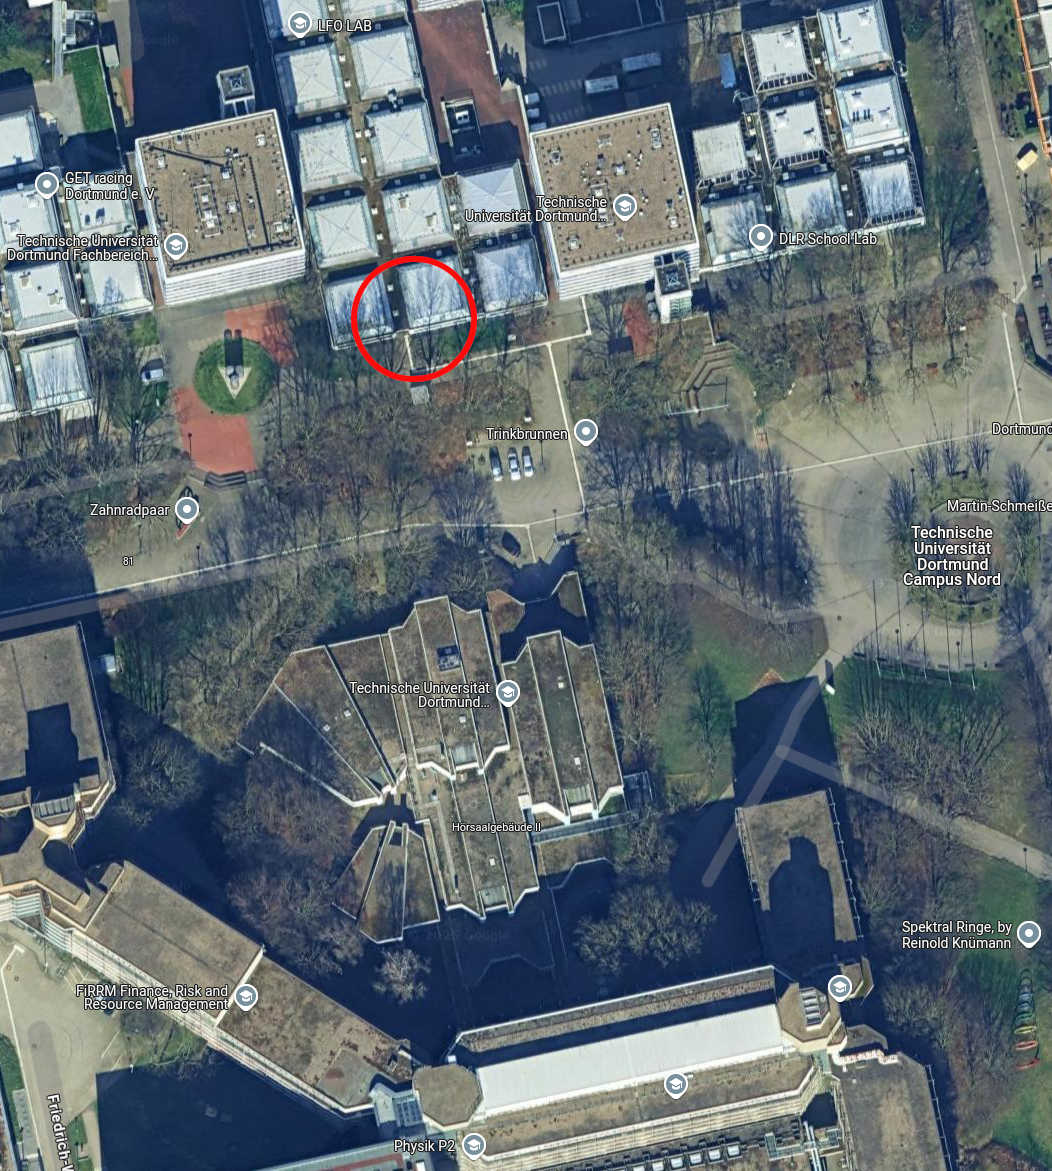
\includegraphics[width=\textwidth]{Lageplan_EF68.jpg}
  \end{minipage}
\end{frame}

\begin{frame}{Vorbereitung}
  \begin{center}
    \huge
    Auf der Fachschaftsmailingliste eintragen \\
    →~\href{https://mailman.tu-dortmund.de/mailman/listinfo/stud.physik}{mailman.tu-dortmund.de/mailman/listinfo/stud.physik}\\[0.5\baselineskip]
    Anmeldung ausfüllen\\
    →~\textcolor{blue!70!black}{\href{https://registration.pep-dortmund.org/events/toolbox25/registration/}{registration.pep-dortmund.org/events/toolbox25/registration}}\\[0.5\baselineskip]
    Software installieren\\
    →~\textcolor{blue!70!black}{\href{https://toolbox.pep-dortmund.org/install/install/}{toolbox.pep-dortmund.org/install}}\\[0.5\baselineskip]
    Laptops/Rechner vorbereiten + mitbringen/uns ansprechen
  \end{center}
\end{frame}
\begin{frame}{Neuer Laptop oder anderes Betriebssystem?}
  \huge
  Neuen Laptop kaufen? \newline
  Denkt über ein amerikanisches Tastaturlayout nach\\[0.5\baselineskip]

  Falls ihr euch für Linux interessiert:
	\begin{itemize}
		\item ressourcenschonend (gut für ältere Laptops)
		\item einfache Installation von wissenschaftlichen Standardtools
		\item Standard auf Servern
		\item Open Source
	\end{itemize}
\end{frame}
\begin{frame}{Installation}
  \huge
  Falls ihr Linux installieren wollt:\\[0.5\baselineskip]
	\begin{enumerate}[a)]
    \item Unserer \href{https://toolbox.pep-dortmund.org/install/dualboot/}{Anleitung} folgen.
    \item oder mit persönlicher Anleitung:
  \end{enumerate}
  \begin{itemize}
    \item In der Anmeldung mit angeben
    \item zusätzlich gerne eine Mail an \href{mailto:pep-toolbox.physik@lists.tu-dortmund.de}{pep-toolbox.physik@lists.tu-dortmund.de}
    \item Donnerstag 25.09.2025: ab 10:00 Uhr, Ort: CP-03-123
  \end{itemize}
\end{frame}
\begin{frame}
  \begin{minipage}{.5\textwidth}
    \Huge\centering
    \textcolor{red!70!black}{Fragen?}
  \end{minipage}
  \begin{minipage}{.49\textwidth}
    \centering
    \includegraphics[width=.8\textwidth]{../qrcode/toolbox_qrcode.png}
    \Large
    \href{https://toolbox.pep-dortmund.org}{\textcolor{darkgray}{\texttt{toolbox.pep-dortmund.org}}}
  \end{minipage}
\end{frame}
\end{document}
